\chapter{MOLECULAR DYNAMICS SIMULATIONS OF THE SURFACE RECONSTRUCTIONS OF PT(557) AND AU(557) UNDER EXPOSURE TO CO}
\label{chap:PtAu}


%\begin{abstract}
%  The mechanism and dynamics of surface reconstructions of Pt(557) and
%  Au(557) exposed to various coverages of carbon monoxide (CO) were
%  investigated using molecular dynamics simulations.  Metal-CO
%  interactions were parameterized from experimental data and
%  plane-wave Density Functional Theory (DFT) calculations.  The large
%  difference in binding strengths of the Pt-CO and Au-CO interactions
%  was found to play a significant role in step-edge stability and
%  adatom diffusion constants.  Various mechanisms for CO-mediated step
%  wandering and step doubling were investigated on the Pt(557)
%  surface.  We find that the energetics of CO adsorbed to the surface
%  can explain the step-doubling reconstruction observed on Pt(557) and
%  the lack of such a reconstruction on the Au(557) surface.  However,
%  more complicated reconstructions into triangular clusters that have
%  been seen in recent experiments were not observed in these
%  simulations.
%\end{abstract}

%\newpage


In this chapter I report on simulations of \ce{Pt} and \ce{Au} (557) surfaces
exposed to various coverages of \ce{CO}. The effect of \ce{CO}-\ce{CO}
repulsion is examined as a possible cause for experimentally observed
step-doubling of the \ce{Pt} (557) system. The strong \ce{Pt\bond{-}CO} bond is
also believed to play a role. The \ce{Au\bond{-}CO} interaction is
significantly weaker suggesting a cause for the reduced reconstruction on the
\ce{Au} surface. These simulations require an accurate description of cross
interactions between the metal and \ce{CO} and forcefields describing these
interactions have been parameterized as part of this work. An in-depth
examination of surface dynamics focusing on adatom mobility is also performed.



%\section{Introduction}

%Industrial catalysts usually consist of small particles that exhibit a
%high concentration of steps, kink sites, and vacancies at the edges of
%the facets.  These sites are thought to be the locations of catalytic
%activity.\citep{Jeong:1999ev, Larsen:1999le} There is now
%significant evidence that solid surfaces are often structurally,
%compositionally, and chemically modified by reactants under operating
%conditions.\citep{Tao:2008aa, Tao:2010aa, Tao:2011aa} The coupling between
%surface oxidation states and catalytic activity for CO oxidation on
%Pt, for instance, is widely documented.\citep{Ertl:2008nz, Hendriksen:2002ay}
%Despite the well-documented role of these effects on reactivity, the
%ability to capture or predict them in atomistic models is somewhat
%limited.  While these effects are perhaps unsurprising on the highly
%disperse, multi-faceted nanoscale particles that characterize
%industrial catalysts, they are manifest even on ordered, well-defined
%surfaces. The Pt(557) surface, for example, exhibits substantial and
%reversible restructuring under exposure to moderate pressures of
%carbon monoxide.\citep{Tao:2010aa}

%This work is an investigation into the mechanism and timescale for the
%Pt(557) \& Au(557) surface restructuring using molecular simulation.
%Since the dynamics of the process are of particular interest, we
%employ classical force fields that represent a compromise between
%chemical accuracy and the computational efficiency necessary to
%simulate the process of interest.  Since restructuring typically
%occurs as a result of specific interactions of the catalyst with
%adsorbates, in this work, two metal systems exposed to carbon monoxide
%were examined. The Pt(557) surface has already been shown to undergo a
%large scale reconstruction under certain conditions.\citep{Tao:2010aa}
%The Au(557) surface, because of weaker interactions with CO, is less
%likely to undergo this kind of reconstruction. However, Peters {\it et
%  al}.\citep{Peters:2000zh} and Piccolo {\it et al}.\citep{Piccolo:2004os}
%have both observed CO-induced modification of reconstructions to the
%Au(111) surface. Peters {\it et al}. observed the Au(111)-($22 \times
%\sqrt{3}$) ``herringbone'' reconstruction relaxing slightly under CO
%adsorption. They argued that only a few Au atoms become adatoms,
%limiting the stress of this reconstruction, while allowing the rest to
%relax and approach the ideal (111) configuration.  Piccolo {\it et
%  al}. on the other hand, saw a more significant disruption of the
%Au(111)-($22 \times \sqrt{3}$) herringbone pattern as CO adsorbed on
%the surface. Both groups suggested that the preference CO shows for
%low-coordinated Au atoms was the primary driving force for the
%relaxation.  Although the Au(111) reconstruction was not the primary
%goal of our work, the classical models we have fit may be of future
%use in simulating this reconstruction.

%Platinum molecular dynamics
%gold molecular dynamics

\section{Simulation Methods}
The challenge in modeling any solid/gas interface is the development
of a sufficiently general yet computationally tractable model of the
chemical interactions between the surface atoms and adsorbates.  Since
the interfaces involved are quite large (10$^3$ - 10$^4$ atoms), have
many electrons, and respond slowly to perturbations, {\it ab initio}
molecular dynamics
(AIMD),\citep{Kresse:1993ve, Kresse:1993qf, Kresse:1994ul} Car-Parrinello
methods,\citep{Car:1985bh, Izvekov:2000fv, Guidelli:2000fy} and quantum
mechanical potential energy surfaces remain out of reach.
Additionally, the ``bonds'' between metal atoms at a surface are
typically not well represented in terms of classical pairwise
interactions in the same way that bonds in a molecular material are,
nor are they captured by simple non-directional interactions like the
Coulomb potential.  For this work, we have used classical molecular
dynamics with potential energy surfaces that are specifically tuned
for transition metals.  In particular, we used the EAM potential for
Au-Au and Pt-Pt interactions.\citep{Foiles:1986ky} The CO was modeled using
a rigid three-site model developed by Straub and Karplus for studying
photodissociation of CO from myoglobin.\citep{Straub:1991no} The Au-CO and
Pt-CO cross interactions were parameterized as part of this work.
  
\subsection{Metal-metal interactions}
Many of the potentials used for modeling transition metals are based
on a non-pairwise additive functional of the local electron
density. The embedded atom method (EAM) is perhaps the best known of
these
methods,\citep{Foiles:1986ky, Daw:1984aq, Johnson:1989yr, Daw:1989ci, Plimpton:1993qi, Voter:1995ax, Lu:1997fv, Alemany:1998fp}
but other models like the Finnis-Sinclair\citep{Finnis:1984hl, Sutton:1990rr} and
the quantum-corrected Sutton-Chen method\citep{Goddard:1998qsc, Qi:1999dn} have simpler
parameter sets. The glue model of Ercolessi {\it et
  al}.\citep{Ercolessi:1988uo} is among the fastest of these density
functional approaches. In all of these models, atoms are treated as a
positively charged core with a radially-decaying valence electron
distribution. To calculate the energy for embedding the core at a
particular location, the electron density due to the valence electrons
at all of the other atomic sites is computed at atom $i$'s location,
\begin{equation*}
\bar{\rho}_i = \sum_{j\neq i} \rho_j(r_{ij})
\end{equation*}
Here, $\rho_j(r_{ij})$ is the function that describes the distance
dependence of the valence electron distribution of atom $j$. The
contribution to the potential that comes from placing atom $i$ at that
location is then
\begin{equation*}
V_i =  F[ \bar{\rho}_i ]  + \sum_{j \neq i} \phi_{ij}(r_{ij})
\end{equation*}
where $F[ \bar{\rho}_i ]$ is an energy embedding functional, and
$\phi_{ij}(r_{ij})$ is a pairwise term that is meant to represent the
repulsive overlap of the two positively charged cores.  

% The {\it modified} embedded atom method (MEAM) adds angular terms to
% the electron density functions and an angular screening factor to the
% pairwise interaction between two
% atoms.\citep{BASKES:1994fk,Lee:2000vn,Thijsse:2002ly,Timonova:2011ve}
% MEAM has become widely used to simulate systems in which angular
% interactions are important (e.g. silicon,\citep{Timonova:2011ve} bcc
% metals,\citep{Lee:2001qf} and also interfaces.\citep{Beurden:2002ys})
% MEAM presents significant additional computational costs, however.

The EAM, Finnis-Sinclair, and the Quantum Sutton-Chen (QSC) potentials
have all been widely used by the materials simulation community for
simulations of bulk and nanoparticle
properties,\citep{Chui:2003fk, Wang:2005qy, Medasani:2007uq, Mishin:1999ew}
melting,\citep{Belonoshko:2000jk, Sankaranarayanan:2006ye, Sankaranarayanan:2005bh}
fracture,\citep{Shastry:1996qg, Shastry:1998dx, Mishin:2001qt} crack
propagation,\citep{Becquart:1993sr, Rifkin:1992ug} and alloying
dynamics.\citep{Shibata:2002hh, Mishin:2002if, Zope:2003ai, Mishin:2005vc}
One of EAM's strengths is its sensitivity to small changes in
structure. This is due to the inclusion of up to the third nearest
neighbor interactions during fitting of the parameters.\citep{Voter:1995ax}
In comparison, the glue model of Ercolessi {\it et
  al}.\citep{Ercolessi:1988uo} was only parameterized to include
nearest-neighbor interactions. EAM is a suitable choice for systems
where the bulk properties are of secondary importance to low-index
surface structures. Additionally, the similarity of EAM's functional
treatment of the embedding energy to standard density functional
theory (DFT) makes fitting DFT-derived cross potentials with
adsorbates somewhat easier.

\subsection{Carbon monoxide model}
Previous explanations for the surface rearrangements center on the
large linear quadrupole moment of carbon monoxide.\citep{Tao:2010aa} We
used a model first proposed by Karplus and Straub to study the
photodissociation of CO from myoglobin because it reproduces the
quadrupole moment well.\citep{Straub:1991no} The Straub and Karplus model
treats CO as a rigid three site molecule with a massless
charge-carrying ``M'' site at the center of mass. The geometry and
interaction parameters are reproduced in Table~\ref{tab:CO}. The
effective dipole moment, calculated from the assigned charges, is
still small (0.35 D) while the linear quadrupole (-2.40 D~\AA) is
close to the experimental (-2.63 D~\AA)\citep{Chetty:2011dp} and quantum
mechanical predictions (-2.46 D~\AA)\citep{Rizzo:2000sp}.

%CO Table
\begin{table}[H]
\caption{POSITIONS, LENNARD-JONES PARAMETERS ($\sigma$ AND $\epsilon$), AND
CHARGES FOR CO-CO INTERACTIONS}
\centering
\begin{threeparttable}
%  \caption{Positions, Lennard-Jones parameters ($\sigma$ and
%    $\epsilon$), and charges for CO-CO 
%    interactions. Distances are in \AA, energies are 
%    in kcal/mol, and charges are in atomic units.  The CO model
%    from Ref.\bibpunct{}{}{,}{n}{}{,}
%    \protect\citep{Straub} was used without modification.}
\centering
\begin{tabular}{ c  c  ccc }
\hline \hline
&  {\it z}\tnote{a} & $\sigma$\tnote{a} & $\epsilon$\tnote{b} & q\tnote{c}\\
\hline
\textbf{C} & -0.6457 &  3.83 & 0.0262   &   -0.75 \\
\textbf{O} &  0.4843 &  3.12 &  0.1591  &   -0.85 \\
\textbf{M} & 0.0 & -  &  -  &    1.6 \\
\hline \hline
\end{tabular}
\begin{tablenotes}
  \item The CO model from Ref.\citep{Straub:1991no} was used without modification.
  \item[a] Distances are in \AA.
  \item[b] Energies are in kcal/mol.
  \item[c] Charges are in a.u.
\end{tablenotes}
\end{threeparttable}
\label{tab:CO}
\end{table}

\subsection{Cross-Interactions between the metals and carbon monoxide}

Since the adsorption of CO onto a Pt surface has been the focus
of much experimental \citep{Ertl:1977cg, Kelemen:1979ad, Yeo:1997th, Hopster:1978yf}
and theoretical work
\citep{Deshlahra:2009wu, Feibelman:2001qa, Beurden:2002ys, Korzeniewski:1986kl, Mason:2004ix}
there is a significant amount of data on adsorption energies for CO on
clean metal surfaces. An earlier model by Korzeniewski {\it et
  al.}\citep{Korzeniewski:1986kl} served as a starting point for our fits. The parameters were
modified to ensure that the Pt-CO interaction favored the atop binding
position on Pt(111). These parameters are reproduced in Table~\ref{tab:co_parameters}.
The modified parameters yield binding energies that are slightly higher
than the experimentally-reported values as shown in Table~\ref{tab:co_energies}. Following Korzeniewski
{\it et al}.,\citep{Korzeniewski:1986kl} the Pt-C interaction was fit to a deep
Lennard-Jones interaction to mimic strong, but short-ranged, partial
binding between the Pt $d$ orbitals and the $\pi^*$ orbital on CO. The
Pt-O interaction was modeled with a Morse potential with a large
equilibrium distance, ($r_o$).  These choices ensure that the C is preferred
over O as the surface-binding atom. In most geometries, the Pt-O parameterization contributes a weak
repulsion which favors the atop site.  The resulting potential-energy
surface suitably recovers the calculated Pt-C separation length
(1.6~\AA)\citep{Beurden:2002ys} and affinity for the atop binding
position.\citep{Deshlahra:2012aa, Hopster:1978yf}

%where did you actually get the functionals for citation?
%scf calculations, so initial relaxation was of the four layers, but two layers weren't kept fixed, I don't think
%same cutoff for slab and slab + CO ? seems low, although feibelmen had values around there...
The Au-C and Au-O cross-interactions were also fit using Lennard-Jones and
Morse potentials, respectively, to reproduce Au-CO binding energies.
The limited experimental data for CO adsorption on Au required refining the fits against plane-wave DFT calculations.
Adsorption energies were obtained from gas-surface DFT calculations with a
periodic super-cell plane-wave basis approach, as implemented in the
Quantum ESPRESSO package.\citep{Giannozzi:2009fe} Electron cores were
described with the projector augmented-wave (PAW)
method,\citep{Blochl:1994vf, Kresse:1999by} with plane waves
included to an energy cutoff of 20 Ry. Electronic energies are
computed with the PBE implementation of the generalized gradient
approximation (GGA) for gold, carbon, and oxygen that was constructed
by Rapp\'e, Rabe, Kaxiras, and Joannopoulos.\citep{Perdew:1996fq, Rappe:1990tw}
In testing the Au-CO interaction, Au(111) super-cells were constructed of four layers of 4
Au x 2 Au surface planes and separated from vertical images by six
layers of vacuum space. The surface atoms were all allowed to relax 
before CO was added to the system. Electronic relaxations were 
performed until the energy difference between subsequent steps 
was less than $10^{-8}$ Ry.   Nonspin-polarized super-cell calculations 
were performed with a 4~x~4~x~4 Monkhorst-Pack {\bf k}-point sampling of the first Brillouin
zone.\citep{Monkhorst:1976il} The relaxed gold slab was
then used in numerous single point calculations with CO at various
heights (and angles relative to the surface) to allow fitting of the
empirical force field.

%Hint at future work
The parameters employed for the metal-CO cross-interactions in this work 
are shown in Table~\ref{tab:co_parameters} and the binding energies on the 
(111) surfaces are displayed in Table~\ref{tab:co_energies}.  Charge transfer
and polarization are neglected in this model, although these effects could have 
an effect on binding energies and binding site preferences.

%Table  of Parameters
%Pt Parameter Set 9
%Au Parameter Set 35
\begin{table}[H]
  \caption{PARAMETERS FOR THE METAL-CO CROSS-INTERACTIONS}
%  \caption{Parameters for the metal-CO cross-interactions. Metal-C
%    interactions are modeled with Lennard-Jones potentials, while the
%    metal-O interactions were fit to broad Morse
%    potentials.  Distances are given in \AA~and energies in kcal/mol. }
\centering
\begin{threeparttable}
\begin{tabular}{  c   cc   c  ccc }
\hline \hline
 &  $\sigma$\tnote{a} & $\epsilon$\tnote{b} & & $r$\tnote{a} & $D$\tnote{b} & $\gamma$ (\AA$^{-1}$) \\
\hline
\textbf{Pt-C} & 1.3 & 15  & \textbf{Pt-O} & 3.8 & 3.0 & 1 \\
\textbf{Au-C} & 1.9 & 6.5  & \textbf{Au-O} & 3.8 & 0.37 & 0.9\\
\hline \hline
\end{tabular}
\begin{tablenotes}
  \item Metal-C interactions are modeled with Lennard-Jones potentials, while the metal-O interactions were fit to broad Morse potentials.
  \item[a] Distances are given in \AA
  \item[b] Energies are given in kcal/mol
\end{tablenotes}
\end{threeparttable}
\label{tab:co_parameters}
\end{table}

%Table of energies
\begin{table}[H]
%  \caption{Adsorption energies for a single CO at the atop site on M(111) using
%the potentials described in this work.  All values are in eV.}
\caption{ADSORPTION ENERGIES FOR CO ON M(111)}
\centering
\begin{threeparttable}
\begin{tabular}{ c  cc }
  \hline \hline
  & Calculated\tnote{a} & Experimental\tnote{a} \\
  \hline
%  \multirow{2}{*}{\textbf{Pt-CO}} & \multirow{2}{*}{-1.81} & -1.4 \bibpunct{}{}{,}{n}{}{,}
%  (Ref. \protect\citep{Kelemen:1979}) \\
% & &  -1.9 \bibpunct{}{}{,}{n}{}{,} (Ref. \protect\citep{Yeo}) \\ \hline
%  \textbf{Au-CO} & -0.39 & -0.40 \bibpunct{}{}{,}{n}{}{,}  (Ref. \protect\citep{TPDGold}) \\
  \multirow{2}{*}{\textbf{Pt-CO}} & \multirow{2}{*}{-1.81} & -1.4
  Ref. \citep{Kelemen:1979ad} \\
 & &  -1.9 Ref. \citep{Yeo:1997th} \\ \hline
  \textbf{Au-CO} & -0.39 & -0.40 Ref. \citep{Elliott:1984zt} \\
  \hline \hline
\end{tabular}
\begin{tablenotes}
  \item The adsorption energies were calculated for a single CO molecule
adsorbed vertically at an atop binding site on a (111) metal surface using the
potentials described in this work 
  \item[a] Adsorption energies are given in eV
\end{tablenotes}
\end{threeparttable}
\label{tab:co_energies}
\end{table}


\subsection{Force field validation}
The CO-Pt cross interactions were compared directly to DFT results
found in the supporting information of reference
\citep{Tao:2010aa}. These energies are
estimates of the degree of stabilization provided to double-layer
reconstructions of the M(557) surface by an overlayer of CO molecules
in a $c (2 \times 4)$ pattern.  To make the comparison, five atom
thick metal slabs of both Pt and Au displaying the (557) facet were
constructed.  Double-layer (reconstructed) systems were created using
six atomic layers where enough of a layer was removed from both
exposed (557) facets to create the double step.  In all cases, the
metal slabs contained 480 atoms and were minimized using steepest
descent under the EAM force field. Both the bare metal slabs and slabs
with 50\% carbon monoxide coverage (arranged in the $c (2 \times 4)$
pattern) were used.  The systems are periodic along and perpendicular
to the step-edge axes with a large vacuum above the displayed (557)
facet.

Energies computed using our force field are displayed in Table
~\ref{tab:steps}.  The relative energies are calculated as
$E_{relative} = E_{system} - E_{M(557)-S} - N_{CO}*E_{M-CO}(r)$, where
$E_{M(557)-S}$ is the energy of a clean (557) surface. $N_{CO}$ is the
number of CO molecules present on the surface.  In the $c (2 \times
4)$ patterning, the CO molecules relax to an average separation, $r$,
from the nearest surface metal atom.  $E_{M-CO}(r)$ is taken as the
energy of a single CO molecule on a flat M(111) surface at a distance
$r$ from a metal atop site.  These energies correspond to -1.8 eV for
CO-Pt and -0.39 eV for CO-Au. 

One important note is that the $c (2 \times 4)$ patterning on the
stepped surfaces yields a slightly larger M-CO separation than one
would find on a clean (111) surface. On a clean Pt(111) surface, for
example, the optimized geometry has a C-Pt distance of 1.53~\AA
(corresponding to a binding energy of -1.83 eV).  On the double-layer
reconstruction and the single (557) step, the half monolayer optimizes
to C-Pt separations of 1.58-1.60~\AA, respectively.  Although this
difference seems quite small, there are notable consequences for
$E_{Pt-CO}(r)$ which then takes values from -1.815 eV to -1.8 eV.

For platinum, the bare double layer reconstruction is less stable than
the bare (557) step by about 0.25 kcal/mol per Pt atom. However,
addition of carbon monoxide changes the relative energetics of the two
systems. This is a quite dramatic shift, $\Delta\Delta E$ (the change
in energy for going from single to double-layer structures upon
addition of a CO layer) shifts by -0.5~kcal/mol per Pt atom. This
result is in qualitative agreement with the DFT calculations in
reference \citep{Tao:2010aa}, which
also showed that the addition of CO leads to a reversal in stability.

The gold systems show a smaller energy difference between the clean
single and double layers. Upon addition of CO, the single step surface
is much more stable than the double-layer reconstruction.  However,
the CO-Au binding energy is much weaker, so at operating temperatures,
the actual coverage by CO will be much lower than the 50\% coverage
afforded by the $c (2 \times 4)$ pattern, so single-point energy
comparisons are not as helpful.

%Table of single step double step calculations
\begin{table}
\caption{RELATIVE ENERGIES OF (S)INGLE M(557) AND (D)OUBLE-STEP RECONSTRUCTIONS}
%  \caption{Relative energies (in kcal/mol) of (S)ingle M(557) and
%    (D)ouble-step reconstructions. 50\% coverage by CO in a  $c(2
%    \times 4)$ pattern stabilizes the D-reconstructed Pt(557)
%    surface, but leaves the single-step Au(557) as the more stable structure.}
\centering
\begin{threeparttable}
\centering
\begin{tabular}{  c   c   c   c   c  }
\hline \hline
Step & $N_{M}$ & $N_{CO}$ & Relative Energy & $\Delta E / N_{M}$ \\
\hline
Pt(557)-S & 480 & 0  &  0 & 0 \\
Pt(557)-D & 480 & 0  &  119.788 & 0.2495 \\
Pt(557)-S & 480 & 40 &  -109.734 & -0.2286 \\
Pt(557)-D & 480 & 48 &  -110.039 & -0.2292 \\
\hline
Au(557)-S & 480 & 0  &  0 & 0  \\
Au(557)-D & 480 & 0  &  83.853 & 0.1747 \\
Au(557)-S & 480 & 40 &  -253.604 & -0.5283 \\
Au(557)-D & 480 & 48 &  -156.150 & -0.3253 \\
\hline \hline
\end{tabular}
\begin{tablenotes}
  \item The presence of a 50\% coverage of CO in a $c(2\times 4)$ pattern stabilizes the D-reconstructed Pt(557) surface, but leaves the S-unreconstructed Au(557) as the more stable structure
  \item[a] Energies are in kcal/mol
\end{tablenotes}
\end{threeparttable}
\label{tab:steps}
\end{table}

Qualitatively, our classical force field for the metal-CO cross
interactions reproduces the results predicted by DFT studies in
reference \citep{Tao:2010aa}. Addition
of polarization effects, both in the CO and in the metal surfaces,
could make the model significantly more accurate.  For example,
because of the relatively large fixed charges, the current model will
be unable to reproduce coverages in excess of 50\% without forming an
inverted CO second layer on the surface.  The M-CO cross interactions
would also be more accurate if they included the direct interactions
between charges on the CO and their image charges inside the metal
slab. These polarization effects have been shown to play an important
role,\citep{Deshlahra:2012aa} and would be one way of improving the
numerical agreement with quantum mechanical calculations.

\subsection{Pt(557) and Au(557) metal interfaces}
Our Pt system is an orthorhombic periodic box of dimensions
54.482~x~50.046~x 120.88~\AA, while our Au system has 
dimensions of 57.4~x~51.9285~x~100~\AA. The metal slabs 
are 9 and 8 atoms deep respectively, corresponding to a slab 
thickness of $\sim$21~\AA~ for Pt and $\sim$19~\AA~for Au.
The systems are arranged in a FCC crystal that have been cut
along the (557) plane so that they are periodic in the {\it x} and
{\it y} directions, and have been oriented to expose two aligned
(557) cuts along the extended {\it z}-axis.  Simulations of the 
bare metal interfaces at temperatures ranging from 300~K to
1200~K were performed to confirm the relative
stability of the surfaces without a CO overlayer.  

The different bulk melting temperatures predicted by EAM
(1345~$\pm$~10~K for Au\citep{Ahmed:2003lk} and $\sim$~2045~K for
Pt\citep{Bhattacharya:2011bq}) suggest that any reconstructions should happen at
different temperatures for the two metals.  The bare Au and Pt
surfaces were initially run in the canonical (NVT) ensemble at 800~K
and 1000~K respectively for 100 ps. The two surfaces were relatively
stable at these temperatures when no CO was present, but experienced
increased surface mobility on addition of CO. Each surface was then
dosed with different concentrations of CO that was initially placed in
the vacuum region.  Upon full adsorption, these concentrations
correspond to 0\%, 5\%, 25\%, 33\%, and 50\% surface coverage. Higher
coverages resulted in the formation of a double layer of CO, which
introduces artifacts that are not relevant to (557) reconstruction.
Because of the difference in binding energies, nearly all of the CO
was bound to the Pt surface, while the Au surfaces often had a
significant CO population in the gas phase.  These systems were
allowed to reach thermal equilibrium (over 5~ns) before being run in
the microcanonical (NVE) ensemble for data collection. All of the
systems examined had at least 40~ns in the data collection stage,
although simulation times for some Pt of the systems exceeded 200~ns.
Simulations were carried out using the open source molecular dynamics
package, OpenMD.\citep{Fennell:2006xq, Meineke:2005pt, openmd}


% RESULTS
%
\section{Results}
\subsection{Structural remodeling}
The bare metal surfaces experienced minor roughening of the step-edge
because of the elevated temperatures, but the (557) face was stable
throughout the simulations. The surfaces of both systems, upon dosage
of CO, began to undergo extensive remodeling that was not observed in
the bare systems. Reconstructions of the Au systems were limited to
breakup of the step-edges and some step wandering. The lower coverage
Pt systems experienced similar step edge wandering but to a greater
extent. The 50\% coverage Pt system was unique among our simulations
in that it formed well-defined and stable double layers through step
coalescence, similar to results reported by Tao {\it et
  al}.\citep{Tao:2010aa}

\subsubsection{Step wandering}
The bare surfaces for both metals showed minimal step-wandering at
their respective temperatures. As the CO coverage increased however,
the mobility of the surface atoms, described through adatom diffusion
and step-edge wandering, also increased.  Except for the 50\% Pt
system where step coalescence occurred, the step-edges in the other
simulations preferred to keep nearly the same distance between steps
as in the original (557) lattice, $\sim$13\AA~for Pt and
$\sim$14\AA~for Au.  Previous work by Williams {\it et
  al}.\citep{Williams:1994aa, Williams:1991qd} highlights the repulsion
that exists between step-edges even when no direct interactions are
present in the system. This repulsion is caused by an entropic barrier
that arises from the fact that steps cannot cross over one
another. This entropic repulsion does not completely define the
interactions between steps, however, so it is possible to observe step
coalescence on some surfaces.\citep{Williams:1991qd} The presence and
concentration of adsorbates, as shown in this work, can affect
step-step interactions, potentially leading to a new surface structure
as the thermodynamic equilibrium.

\subsubsection{Double layers}
Tao {\it et al}.\citep{Tao:2010aa} have shown experimentally that the
Pt(557) surface undergoes two separate reconstructions upon CO
adsorption.  The first involves a doubling of the step height and
plateau length.  Similar behavior has been seen on a number of
surfaces at varying conditions, including Ni(977) and
Si(111).\citep{Williams:1994aa, Williams:1991qd, Pearl:2001ca} Of the two systems we
examined, the Pt system showed a greater propensity for reconstruction
because of the larger surface mobility and the greater extent of step
wandering.  The amount of reconstruction was strongly correlated to
the amount of CO adsorbed upon the surface.  This appears to be
related to the effect that adsorbate coverage has on edge breakup and
on the surface diffusion of metal adatoms. Only the 50\% Pt surface
underwent the doubling seen by Tao {\it et al}.\citep{Tao:2010aa} within
the time scales studied here.  Over a longer time scale (150~ns) two
more double layers formed on this surface. Although double layer
formation did not occur in the other Pt systems, they exhibited more
step-wandering and roughening compared to their Au counterparts. The
50\% Pt system is highlighted in Figure \ref{fig:reconstruct} at
various times along the simulation showing the evolution of a double
layer step-edge.

The second reconstruction observed by Tao {\it et al}.\citep{Tao:2010aa}
involved the formation of triangular clusters that stretched across
the plateau between two step-edges. Neither of the simulated metal
interfaces, within the 40~ns time scale or the extended time of 150~ns
for the 50\% Pt system, experienced this reconstruction.

%Evolution of surface
\begin{figure}[p!]
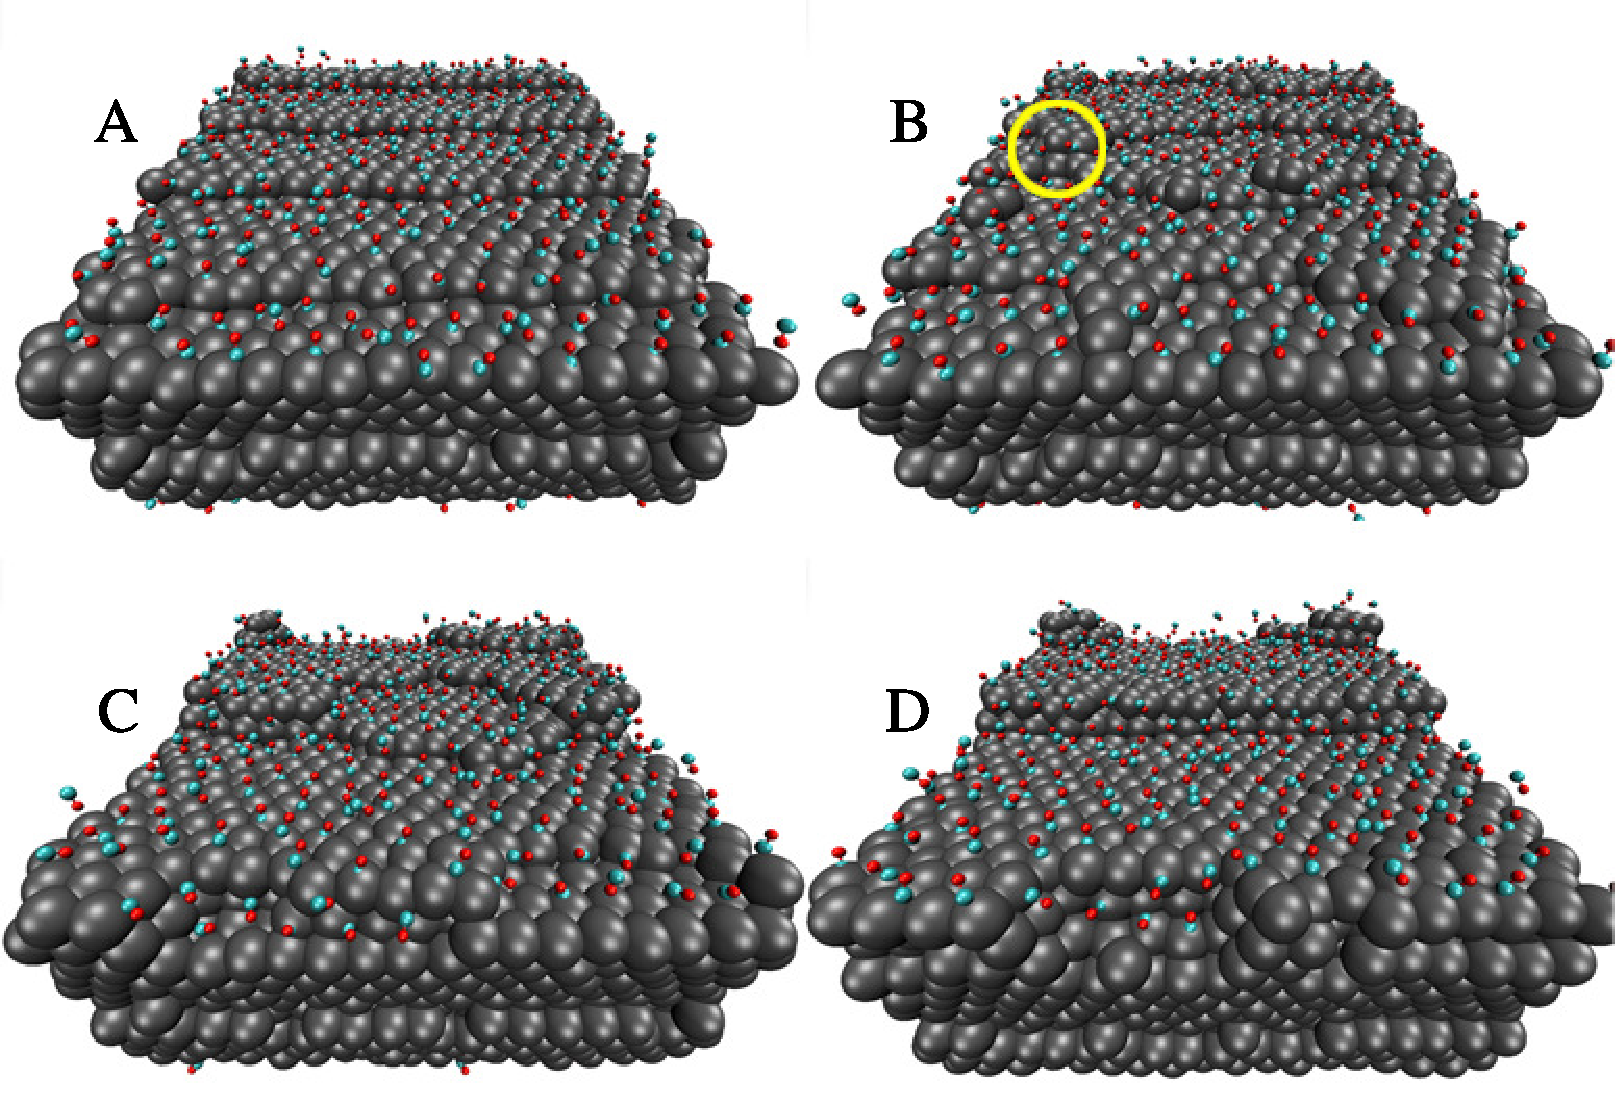
\includegraphics[width=\linewidth]{../figures/chap2/doubleLayer.pdf}
\caption{The Pt(557) / 50\% CO interface upon exposure to the CO: (a)
  258~ps, (b) 19~ns, (c) 31.2~ns, and (d) 86.1~ns after
  exposure. Disruption of the (557) step-edges occurs quickly.  The
  doubling of the layers appears only after two adjacent step-edges
  touch.  The circled spot in (b) nucleated the growth of the double
  step observed in the later configurations.}
  \label{fig:reconstruct}
\end{figure}

\subsection{Dynamics}
Previous experimental work by Pearl and Sibener\citep{Pearl:2001ca}, using
STM, has been able to capture the coalescence of steps on Ni(977). The
time scale of the image acquisition, $\sim$70~s/image, provides an
upper bound for the time required for the doubling to occur. By
utilizing Molecular Dynamics we are able to probe the dynamics of
these reconstructions at elevated temperatures and in this section we
provide data on the timescales for transport properties,
e.g. diffusion and layer formation time.


\subsubsection{Transport of surface metal atoms}
%forcedSystems/stepSeparation

The wandering of a step-edge is a cooperative effect arising from the
individual movements of the atoms making up the steps. An ideal metal
surface displaying a low index facet, (111) or (100), is unlikely to
experience much surface diffusion because of the large energetic
barrier that must be overcome to lift an atom out of the surface. The
presence of step-edges and other surface features on higher-index
facets provides a lower energy source for mobile metal atoms.  Using
our potential model, single-atom break-away from a step-edge on a
clean surface still imposes an energetic penalty around
$\sim$~45~kcal/mol, but this is certainly easier than lifting the same
metal atom vertically out of the surface, \textgreater~60~kcal/mol.
The penalty lowers significantly when CO is present in sufficient
quantities on the surface. For certain distributions of CO, the
energetic penalty can fall to as low as $\sim$~20~kcal/mol. The
configurations that create these lower barriers are detailed in the
discussion section below.

Once an adatom exists on the surface, the barrier for diffusion is
negligible (\textless~4~kcal/mol for a Pt adatom). These adatoms are
then able to explore the terrace before rejoining either their
original step-edge or becoming a part of a different edge. It is an
energetically unfavorable process with a high barrier for an atom to
traverse to a separate terrace although the presence of CO can lower
the energy barrier required to lift or lower an adatom. By tracking
the mobility of individual metal atoms on the Pt and Au surfaces we
were able to determine the relative diffusion constants, as well as
how varying coverages of CO affect the diffusion. Close observation of
the mobile metal atoms showed that they were typically in equilibrium
with the step-edges.  At times, their motion was concerted, and two or
more adatoms would be observed moving together across the surfaces.

A particle was considered ``mobile'' once it had traveled more than
2~\AA~ between saved configurations of the system (typically 10-100
ps). A mobile atom would typically travel much greater distances than
this, but the 2~\AA~cutoff was used to prevent swamping the diffusion
data with the in-place vibrational movement of buried atoms. Diffusion
on a surface is strongly affected by local structures and the presence
of single and double layer step-edges causes the diffusion parallel to
the step-edges to be larger than the diffusion perpendicular to these
edges. Parallel and perpendicular diffusion constants are shown in
Figure \ref{fig:diff}.  Diffusion parallel to the step-edge is higher
than diffusion perpendicular to the edge because of the lower energy
barrier associated with sliding along an edge compared to breaking
away to form an isolated adatom.

%Diffusion graph
\begin{figure}[p!]
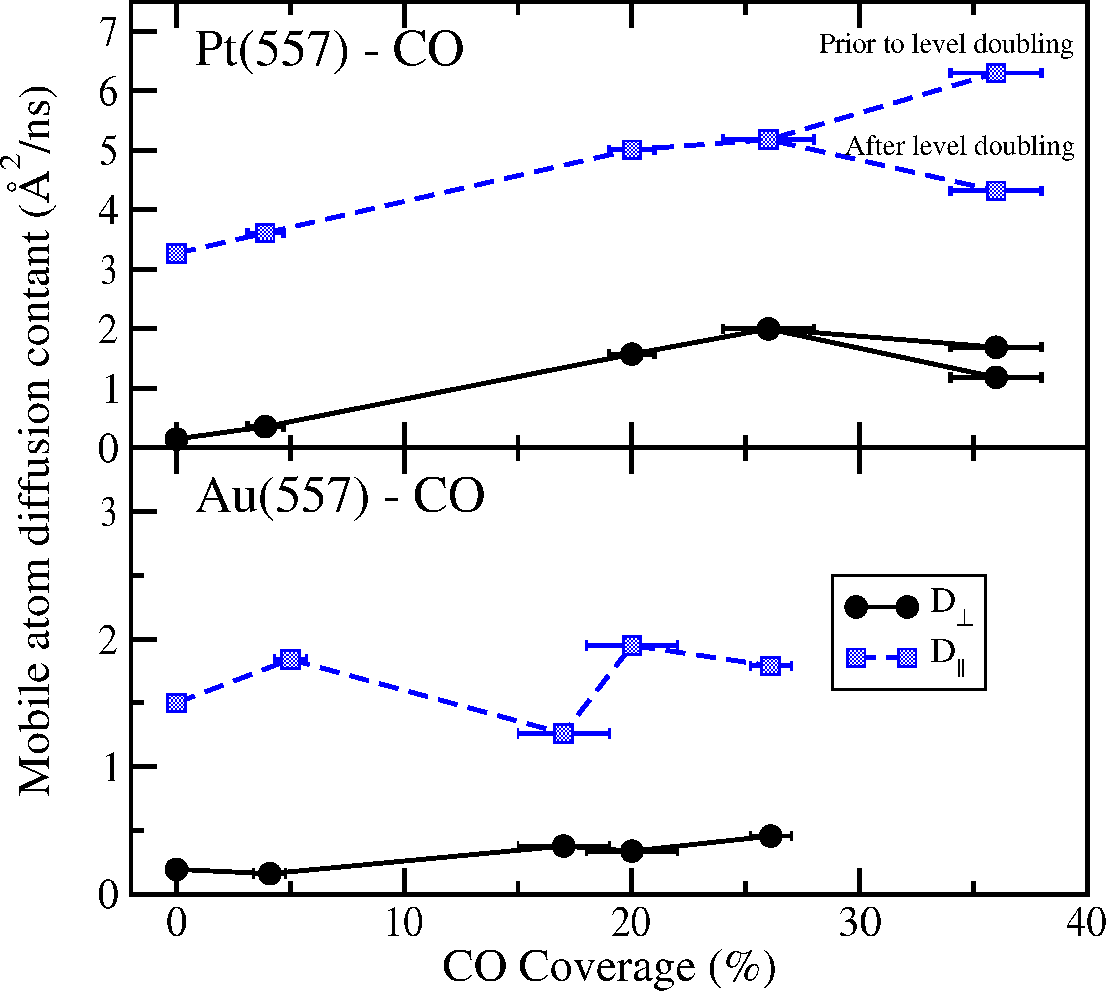
\includegraphics[width=\linewidth]{../figures/chap2/diffusion.pdf}
\caption{Diffusion constants for mobile surface atoms along directions
  parallel ($\mathbf{D}_{\parallel}$) and perpendicular
  ($\mathbf{D}_{\perp}$) to the (557) step-edges as a function of CO
  surface coverage.  The two reported diffusion constants for the 50\%
  Pt system correspond to a 20~ns period before the formation of the
  double layer (upper points), and to the full 40~ns sampling period
  (lower points).}
\label{fig:diff}
\end{figure}

The weaker Au-CO interaction is evident in the weak CO-coverage 
dependence of Au diffusion. This weak interaction leads to lower 
observed coverages when compared to dosage amounts. This further 
limits the effect the CO can have on surface diffusion. The correlation 
between coverage and Pt diffusion rates shows a near linear relationship 
at the earliest times in the simulations. Following double layer formation, 
however, there is a precipitous drop in adatom diffusion. As the double 
layer forms, many atoms that had been tracked for mobility data have 
now been buried, resulting in a smaller reported diffusion constant. A
secondary effect of higher coverages is CO-CO cross interactions that
lower the effective mobility of the Pt adatoms that are bound to each CO.
This effect would become evident only at higher coverages. A detailed
account of Pt adatom energetics follows in the Discussion.
 
\subsubsection{Dynamics of double layer formation}
The increased diffusion on Pt at the higher CO coverages is the primary 
contributor to double layer formation. However, this is not a complete 
explanation -- the 33\%~Pt system has higher diffusion constants, but 
did not show any signs of edge doubling in 40~ns. On the 50\%~Pt 
system, one double layer formed within the first 40~ns of simulation time, 
while two more were formed as the system was allowed to run for an 
additional 110~ns (150~ns total). This suggests that this reconstruction 
is a rapid process and that the previously mentioned upper bound is a 
very large overestimate.\citep{Williams:1991qd,Pearl:2001ca} In this system the first 
appearance of a double layer appears at 19~ns into the simulation. 
Within 12~ns of this nucleation event, nearly half of the step has formed 
the double layer and by 86~ns the complete layer has flattened out. 
From the appearance of the first nucleation event to the first observed 
double layer, the process took $\sim$20~ns. Another $\sim$40~ns was 
necessary for the layer to completely straighten. The other two layers in 
this simulation formed over periods of 22~ns and 42~ns respectively. 
A possible explanation for this rapid reconstruction is the elevated 
temperatures under which our systems were simulated. The process 
would almost certainly take longer at lower temperatures. Additionally, 
our measured times for completion of the doubling after the appearance 
of a nucleation site are likely affected by our periodic boxes. A longer 
step-edge will likely take longer to ``zipper''. 


%Discussion
\section{Discussion}
We have shown that a classical potential is able to model the initial
reconstruction of the Pt(557) surface upon CO adsorption, and have
reproduced the double layer structure observed by Tao {\it et
  al}.\citep{Tao:2010aa}. Additionally, this reconstruction appears to be
rapid -- occurring within 100 ns of the initial exposure to CO.  Here
we discuss the features of the classical potential that are
contributing to the stability and speed of the Pt(557) reconstruction.

\subsection{Diffusion}
The perpendicular diffusion constant appears to be the most important
indicator of double layer formation. As highlighted in Figure
\ref{fig:reconstruct}, the formation of the double layer did not begin
until a nucleation site appeared.  Williams {\it et
  al}.\citep{Williams:1994aa, Williams:1991qd} cite an effective edge-edge
repulsion arising from the inability of edge crossing.  This repulsion
must be overcome to allow step coalescence.  A larger
$\textbf{D}_\perp$ value implies more step-wandering and a larger
chance for the stochastic meeting of two edges to create a nucleation
point.  Diffusion parallel to the step-edge can help ``zipper'' up a
nascent double layer. This helps explain the rapid time scale for
double layer completion after the appearance of a nucleation site, while
the initial appearance of the nucleation site was unpredictable.

\subsection{Mechanism for restructuring}
Since the Au surface showed no large scale restructuring in any of our
simulations, our discussion will focus on the 50\% Pt-CO system which
did exhibit doubling. A number of possible mechanisms exist to explain
the role of adsorbed CO in restructuring the Pt surface. Quadrupolar
repulsion between adjacent CO molecules adsorbed on the surface is one
possibility.  However, the quadrupole-quadrupole interaction is
short-ranged and is attractive for some orientations.  If the CO
molecules are ``locked'' in a vertical orientation, through atop
adsorption for example, this explanation would gain credence. Within
the framework of our classical potential, the calculated energetic
repulsion between two CO molecules located a distance of
2.77~\AA~apart (nearest-neighbor distance of Pt) and both in a
vertical orientation, is 8.62 kcal/mol. Moving the CO to the second
nearest-neighbor distance of 4.8~\AA~drops the repulsion to nearly
0. Allowing the CO to rotate away from a purely vertical orientation
also lowers the repulsion. When the carbons are locked at a distance
of 2.77~\AA, a minimum of 6.2 kcal/mol is reached when the angle
between the 2 CO is $\sim$24\textsuperscript{o}.  The calculated
barrier for surface diffusion of a Pt adatom is only 4 kcal/mol, so
repulsion between adjacent CO molecules bound to Pt could indeed
increase the surface diffusion. However, the residence time of CO on
Pt suggests that the CO molecules are extremely mobile, with diffusion
constants 40 to 2500 times larger than surface Pt atoms. This mobility
suggests that the CO molecules jump between different Pt atoms
throughout the simulation.  However, they do stay bound to individual
Pt atoms for long enough to modify the local energy landscape for the
mobile adatoms.

A different interpretation of the above mechanism which takes the
large mobility of the CO into account, would be in the destabilization
of Pt-Pt interactions due to bound CO.  Destabilizing Pt-Pt bonds at
the edges could lead to increased step-edge breakup and diffusion. On
the bare Pt(557) surface the barrier to completely detach an edge atom
is $\sim$43~kcal/mol, as is shown in configuration (a) in Figures
\ref{fig:SketchGraphic} \& \ref{fig:SketchEnergies}. For certain
configurations, cases (e), (g), and (h), the barrier can be lowered to
$\sim$23~kcal/mol by the presence of bound CO molecules. In these
instances, it becomes energetically favorable to roughen the edge by
introducing a small separation of 0.5 to 1.0~\AA. This roughening
becomes immediately obvious in simulations with significant CO
populations. The roughening is present to a lesser extent on surfaces
with lower CO coverage (and even on the bare surfaces), although in
these cases it is likely due to random fluctuations that squeeze out
step-edge atoms. Step-edge breakup by direct single-atom translations
(as suggested by these energy curves) is probably a worst-case
scenario.  Multistep mechanisms in which an adatom moves laterally on
the surface after being ejected would be more energetically favorable.
This would leave the adatom alongside the ledge, providing it with
five nearest neighbors.  While fewer than the seven neighbors it had
as part of the step-edge, it keeps more Pt neighbors than the three
neighbors an isolated adatom has on the terrace. In this proposed
mechanism, the CO quadrupolar repulsion still plays a role in the
initial roughening of the step-edge, but not in any long-term bonds
with individual Pt atoms.  Higher CO coverages create more
opportunities for the crowded CO configurations shown in Figure
\ref{fig:SketchGraphic}, and this is likely to cause an increased
propensity for step-edge breakup.

%Sketch graphic of different configurations
\begin{figure}[p!]
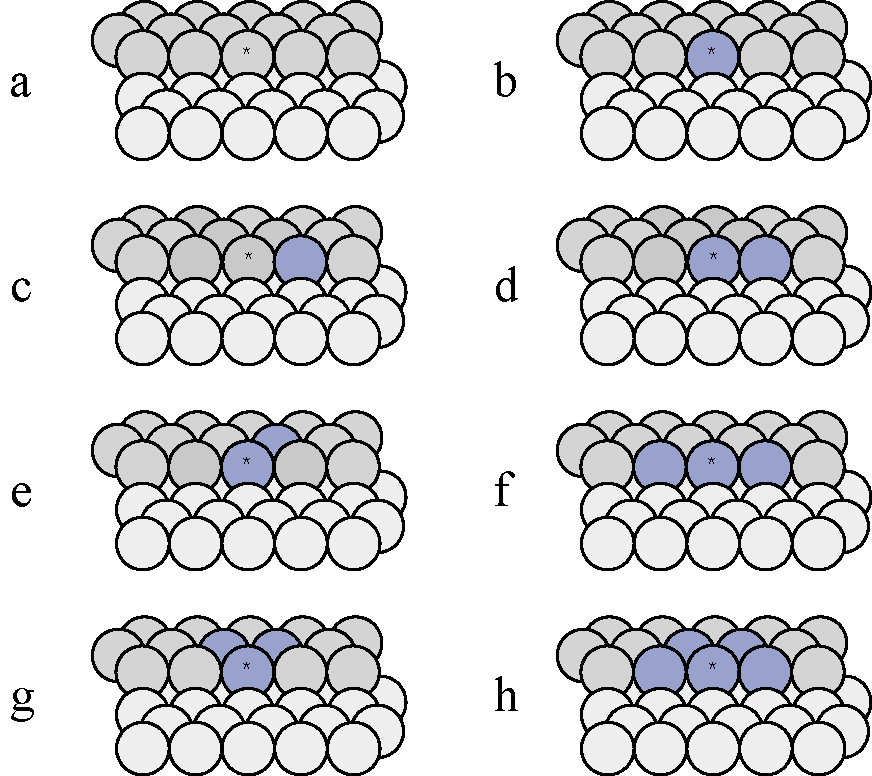
\includegraphics[width=\linewidth]{../figures/chap2/COpaths.pdf}
\caption{Configurations used to investigate the mechanism of step-edge
  breakup on Pt(557). In each case, the central (starred) atom was
  pulled directly across the surface away from the step edge.  The Pt
  atoms on the upper terrace are colored dark grey, while those on the
  lower terrace are in white.  In each of these configurations, some
  of the atoms (highlighted in blue) had CO molecules bound in the
  vertical atop position.  The energies of these configurations as a
  function of central atom displacement are displayed in Figure
  \ref{fig:SketchEnergies}.}
\label{fig:SketchGraphic}
\end{figure}

%energy graph corresponding to sketch graphic
\begin{figure}[p!]
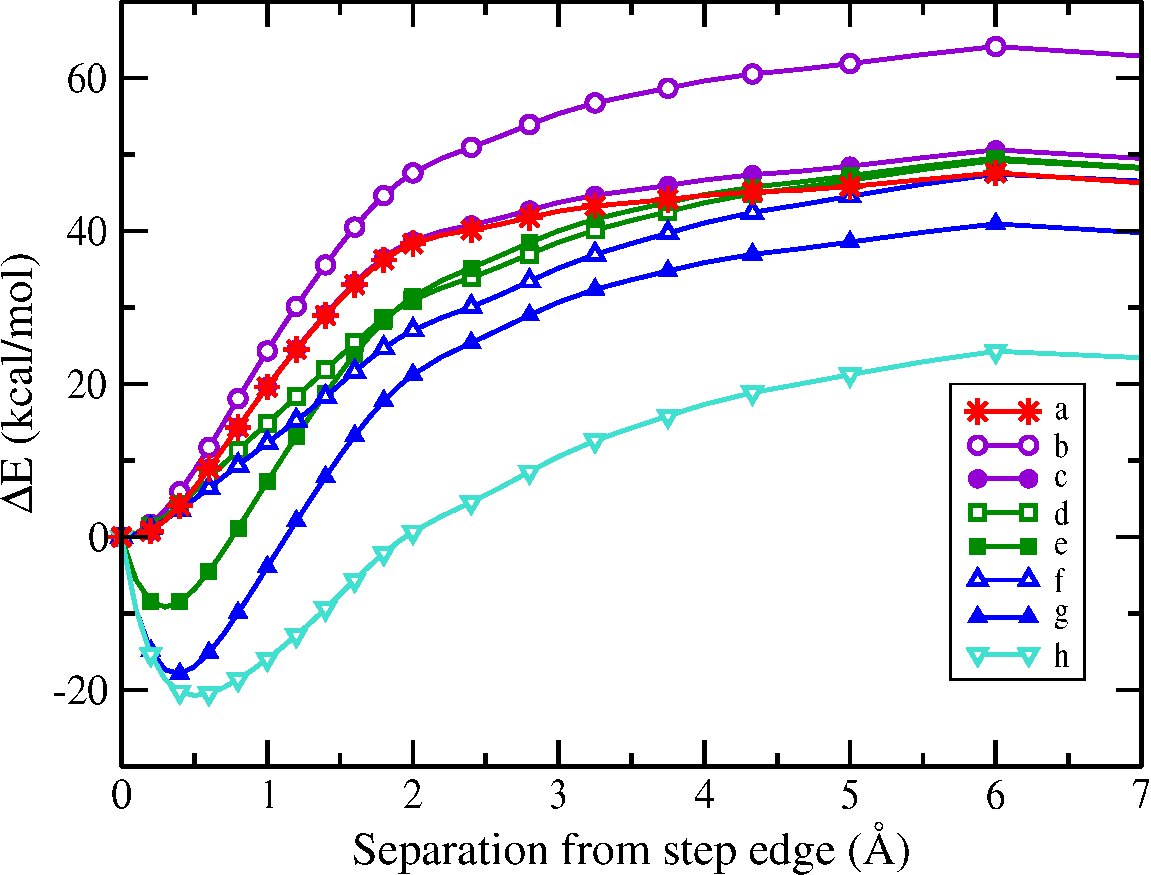
\includegraphics[width=\linewidth]{../figures/chap2/separation.pdf}
\caption{Energies for displacing a single edge atom perpendicular to
  the step edge as a function of atomic displacement. Each of the
  energy curves corresponds to one of the labeled configurations in
  Figure \ref{fig:SketchGraphic}, and the energies are referenced to
  the unperturbed step-edge.  Certain arrangements of bound CO
  (notably configurations g and h) can lower the energetic barrier for
  creating an adatom relative to the bare surface (configuration a).}
\label{fig:SketchEnergies}
\end{figure}

While configurations of CO on the surface are able to increase
diffusion and the likelihood of edge wandering, this does not provide
a complete explanation for the formation of double layers. If adatoms
were constrained to their original terraces then doubling could not
occur.  A mechanism for vertical displacement of adatoms at the
step-edge is required to explain the doubling.

We have discovered one possible mechanism for a CO-mediated vertical
displacement of Pt atoms at the step edge. Figure \ref{fig:lambda}
shows four points along a reaction coordinate in which a CO-bound
adatom along the step-edge ``burrows'' into the edge and displaces the
original edge atom onto the higher terrace.  A number of events
similar to this mechanism were observed during the simulations.  We
predict an energetic barrier of 20~kcal/mol for this process (in which
the displaced edge atom follows a curvilinear path into an adjacent
3-fold hollow site).  The barrier heights we obtain for this reaction
coordinate are approximate because the exact path is unknown, but the
calculated energy barriers would be easily accessible at operating
conditions.  Additionally, this mechanism is exothermic, with a final
energy 15~kcal/mol below the original $\lambda = 0$ configuration.
When CO is not present and this reaction coordinate is followed, the
process is endothermic by 3~kcal/mol.  The difference in the relative
energies for the $\lambda=0$ and $\lambda=1$ case when CO is present
provides strong support for CO-mediated Pt-Pt interactions giving rise
to the doubling reconstruction.

%lambda progression of Pt -> shoving its way into the step
\begin{figure}[p!]
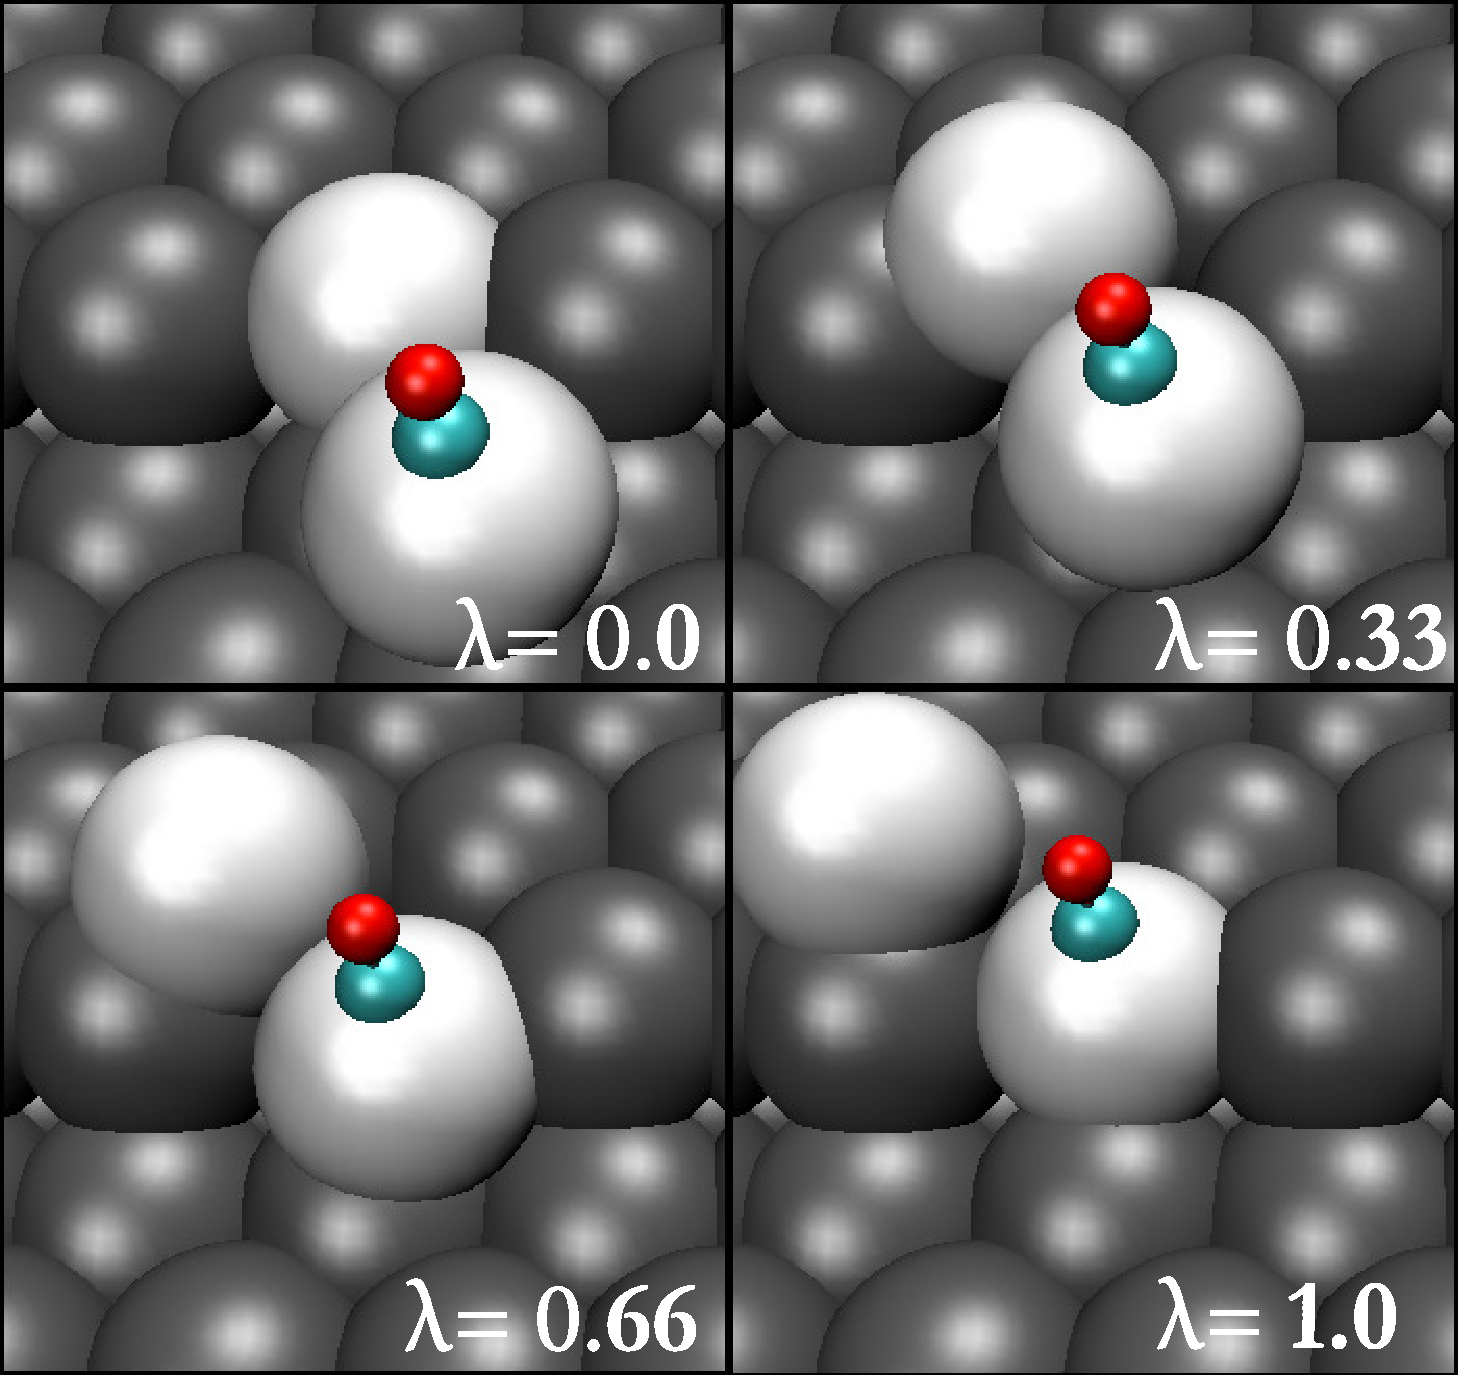
\includegraphics[width=\linewidth]{../figures/chap2/rxn.pdf}
\caption{Points along a possible reaction coordinate for CO-mediated
  edge doubling. Here, a CO-bound adatom burrows into an established
  step edge and displaces an edge atom onto the upper terrace along a
  curvilinear path.  The approximate barrier for the process is
  20~kcal/mol, and the complete process is exothermic by 15~kcal/mol
  in the presence of CO, but is endothermic by 3~kcal/mol without CO.}
\label{fig:lambda}
\end{figure}

The mechanism for doubling on the Pt(557) surface appears to require
the cooperation of at least two distinct processes. For complete
doubling of a layer to occur there must be a breakup of one
terrace. These atoms must then ``disappear'' from that terrace, either
by traveling to the terraces above or below their original levels.
The presence of CO helps explain mechanisms for both of these
situations. There must be sufficient breakage of the step-edge to
increase the concentration of adatoms on the surface and these adatoms
must then undergo the burrowing highlighted above (or a comparable
mechanism) to create the double layer.  With sufficient time, these
mechanisms working in concert lead to the formation of a double layer.

\subsection{CO Removal and double layer stability}
Once the double layers had formed on the 50\%~Pt system, they remained
stable for the rest of the simulation time with minimal movement.
Random fluctuations that involved small clusters or divots were
observed, but these features typically healed within a few
nanoseconds.  Within our simulations, the formation of the double
layer appeared to be irreversible and a double layer was never
observed to split back into two single layer step-edges while CO was
present.

To further gauge the effect CO has on this surface, additional
simulations were run starting from a late configuration of the 50\%~Pt
system that had already formed double layers. These simulations then
had their CO molecules suddenly removed.  The double layer broke apart
rapidly in these simulations, showing a well-defined edge-splitting
after 100~ps. Configurations of this system are shown in Figure
\ref{fig:breaking}. The coloring of the top and bottom layers helps to
show how much mixing the edges experience as they split. These systems
were only examined for 10~ns, and within that time despite the initial
rapid splitting, the edges only moved another few \AA~apart. It is
possible that with longer simulation times, the (557) surface recovery
observed by Tao {\it et al}.\citep{Tao:2010aa} could also be recovered.

\begin{figure}[p!]
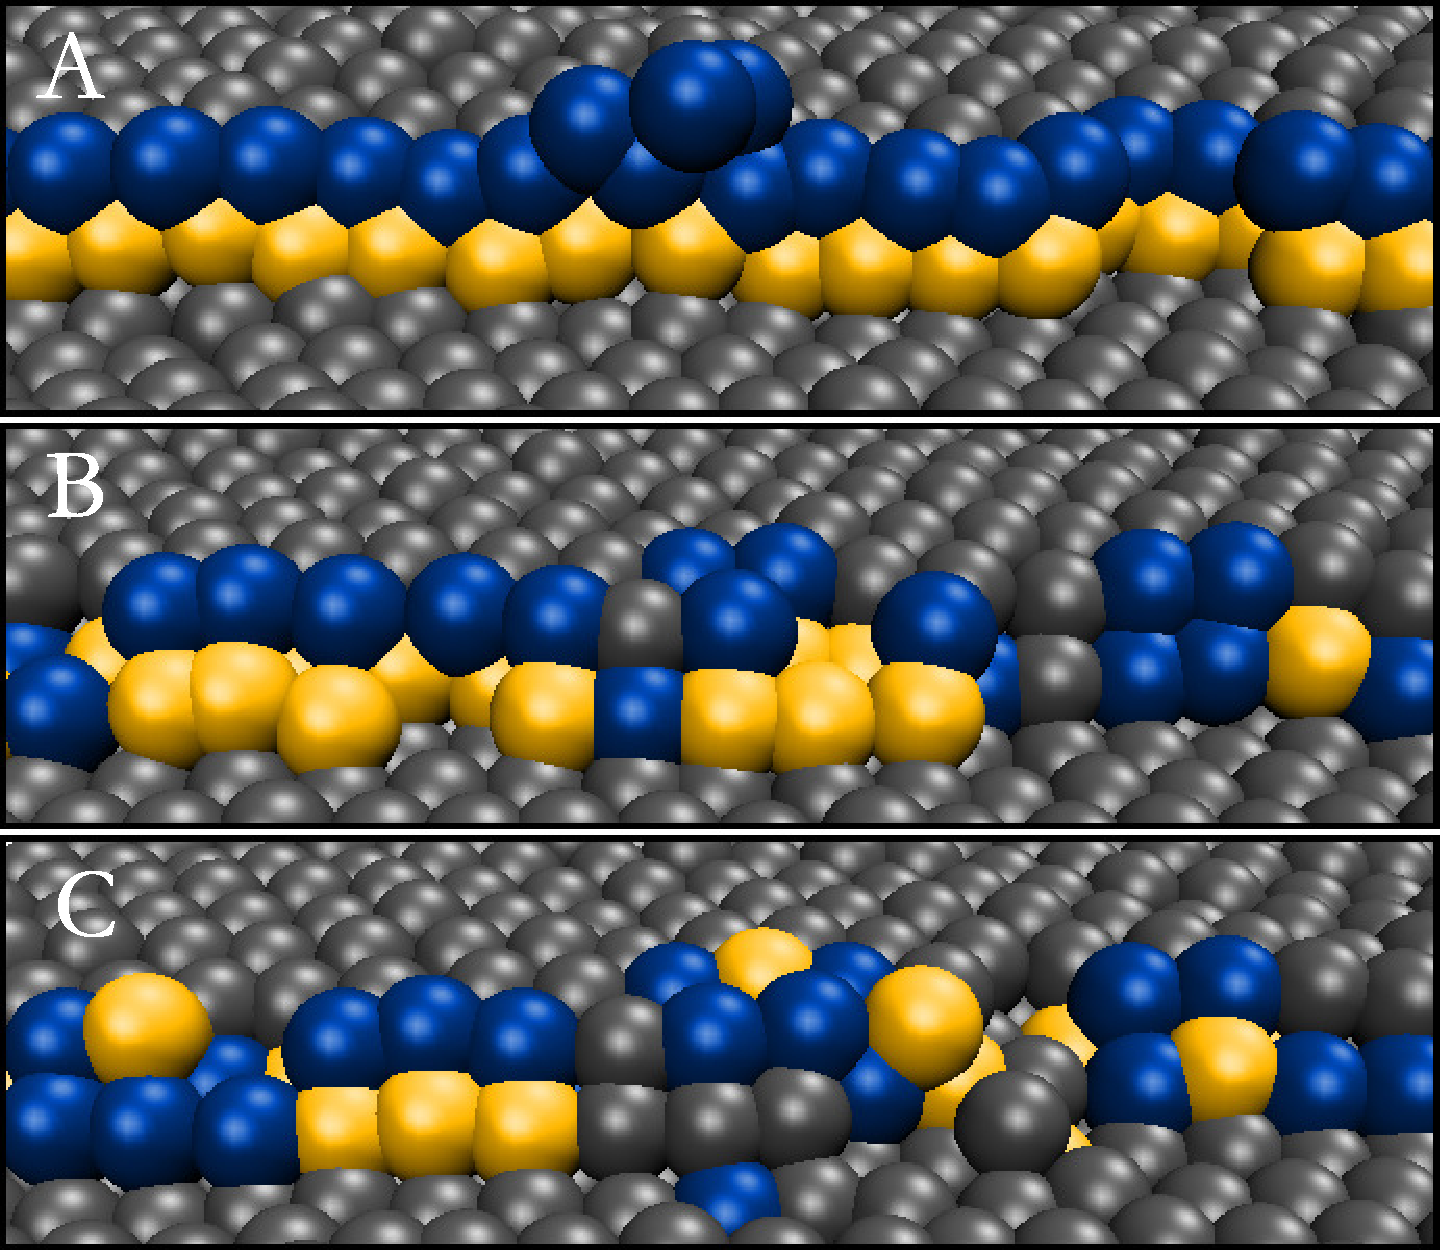
\includegraphics[width=\linewidth]{../figures/chap2/layerBreaking.pdf}
\caption{Behavior of an established (111) double step after removal of
  the adsorbed CO: (A) 0~ps, (B) 100~ps, and (C) 1~ns after the
  removal of CO.  Nearly immediately after the CO is removed, the
  step edge reforms in a (100) configuration, which is also the step
  type seen on clean (557) surfaces. The step separation involves
  significant mixing of the lower and upper atoms at the edge.}
\label{fig:breaking}
\end{figure}


\section{Summary}
We have performed simulations of \ce{Pt} and \ce{Au} (557) systems under a
\ce{CO} atmosphere to identify the mechanism of reconstruction. We showed that
our \ce{Pt\bond{-}CO} forcefield was sufficient to capture the observed
doubling of the \ce{Pt} step-edges. Additionally, we were able to propose a
mechanism based on the strength and directionality of the \ce{Pt\bond{-}CO}
binding interaction, as well as the large quadrupolar repulsion between
atop-bound \ce{CO} molecules to explain the increase in surface mobility. The
weaker \ce{Au\bond{-}CO} interaction resulted in significantly lower adatom
diffusion constants, less step-wandering, and a lack of the double layer
reconstruction on the \ce{Au} (557) surface. An in-depth examination of the
energetics shows the important role \ce{CO} plays in increasing the
step-breakup and in facilitating edge traversal which are both necessary for
double layer formation.


%\section{Conclusion}
%The strength and directionality of the Pt-CO binding interaction, as
%well as the large quadrupolar repulsion between atop-bound CO
%molecules, help to explain the observed increase in surface mobility
%of Pt(557) and the resultant reconstruction into a double-layer
%configuration at the highest simulated CO-coverages.  The weaker Au-CO
%interaction results in significantly lower adataom diffusion
%constants, less step-wandering, and a lack of the double layer
%reconstruction on the Au(557) surface.
%
%An in-depth examination of the energetics shows the important role CO
%plays in increasing step-breakup and in facilitating edge traversal
%which are both necessary for double layer formation.






